\chapter{Colas}

\section{Definición de Cola}
Una cola es una estructura de datos, caracterizada por ser una secuencia de elementos en la que la operación de inserción  se realiza por un extremo y la operación de extracción por el otro. También se le llama estructura FIFO (del inglés First In First Out), debido a que el primer elemento en entrar será también el primero en salir. Este tipo de estructura de datos abstracta se implementa en lenguajes orientados a objetos mediante clases, en forma de nodos enlazados.

La Figura  \ref{fig:cola-representacion} muestra la representación gráfica de una cola con sus operaciones fundamentales de encolar y desencolar.


\begin{figure}
	\centering\textbf{}
		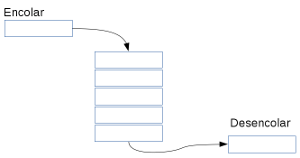
\includegraphics{Diagramas/RepresentacionCola}
	\caption{Representación de una Cola}	
	\label{fig:cola-representacion}
\end{figure}

\begin{definicion}[Cola][capColas:cola]
Una cola es una estructura de datos, caracterizada por ser una secuencia de elementos en la que la operación de inserción  se realiza por un extremo y la operación de extracción por el otro. También se le llama estructura FIFO (del inglés First In First Out), debido a que el primer elemento en entrar será también el primero en salir.
\end{definicion}

\section{El TAD Cola}
A continuación se especifica el TAD de la Cola (al estilo C) con sus operaciones fundamentales. Las operaciones encolar y desencolar son las más importantes. 

\begin{lstlisting}[numbers=none, language=C]
TAD Cola [ T ]
{ invariante: TRUE }
Constructoras:
   crearCola: 
Modificadoras:
	encolar: Cola T 
	desencolar: Cola
Analizadoras:
	frente: Cola
	esVacia: Cola
Destructora:
	destruirCola: Cola

Cola crearCola( void )
/* Crea una cola vacia */
{ post: crearCola = \phi }

void encolar(Cola col, T elem)
/* Agrega elem al final de la cola*/
{ post: col = e1, e2, .. elem}

void desencolar(Cola col)\\
/* Elimina el primer elemento de la cola */
{ pre:  n > 0 }
{ post: col = e2, .., en }

T frente(Cola col )
/* Retorna el primer elemento de la cola */
{ pre: n > 0 }
{ post: frente = e1 }

int esVacia( Cola col )
/* Informa si la cola esta vacia */
 
{ post: esVacia = ( col = \phi) }

void destruirCola( Cola col )
/* Destruye la cola retornando toda la memoria ocupada */
{post: col ha sido destruida }

\end{lstlisting}

\section{Implementación del TAD Cola en Java}
A continuación se muestra una implementación en Java del TAD Cola. Se ha implementado una cola dinámica utilizando nodos enlazados.  Cada nodo almacena un valor y contiene una referencia al siguiente nodo. Supongamos una cola que almacene datos enteros, a la cual se le han aplicado las siguientes operaciones: encolar(10), encolar(35), encolar(12), encolar(7). La Figura \ref{fig:cola-nodos-enlazados} representa cómo quedaría la cola después de encolar en orden los datos 10, 35, 12 y 7. Se puede apreciar que cada nodo almacena un dato y a la vez existe una referencia que almacena la dirección del siguiente nodo. Además, existe una referencia llamada cabeza que apunta al primer elemento que entró (en este caso al dato 10) y una referencia cola que apunta al último dato que entró (o sea el 7).

\begin{figure}
	\centering
	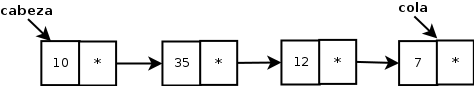
\includegraphics[scale=0.7]{Diagramas/RepresentacionColaNodosEnlazados}
	\caption{Representación de la Cola con Nodos Enlazados}	
	\label{fig:cola-nodos-enlazados}
\end{figure}

La Figura \ref{fig:cola-diagrama-clases} muestra el diagrama de clases que implementa el TAD Cola. Se puede apreciar básicamente dos clases: \textit{Nodo} y \textit{Cola}. La clase \textit{Nodo} representa cada uno de los nodos enlazados que almacenan los objetos que se encolan. Tiene dos atributos,  \textsl{valor} que representa el valor que guarda el nodo, en este caso es una referencia a un objetivo de tipo T (siendo T un tipo genérico). El atributo \textsl{siguiente}, representa la referencia al siguiente nodo. Los demás son únicamente, constructor y getters y setters de cada atributo. A continuación el código fuente de la clase Nodo.


\begin{figure}
	\centering
		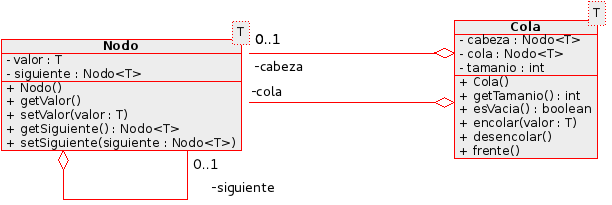
\includegraphics{Diagramas/DiagramaClases-Cola}
	\caption{Diagrama de clase de la implementación del TAD Cola}	
	\label{fig:cola-diagrama-clases}
\end{figure}

\begin{lstlisting}[language=Java]
package co.unicauca.colas;
public class Nodo<T> {
	//Atributo valor de tipo T. Almacena la referencia al objeto que se guarda en el nodo
 	private T valor;
 	//Referencia al siguiente nodo enlazado
 	Nodo<T> siguiente;
	//Constructor por defecto
 	public Nodo() {
 		valor = null;
 		siguiente = null;
 	}
	//Devuelve el valor 
 	public T getValor() {
 		return valor;
 	}
	//Modifica el valor
 	public void setValor(T valor) {
 		this.valor = valor;
 	}
	//Devuelve el atributo siguiente
 	public Nodo<T> getSiguiente() {
 		return siguiente;
 	}
	 //Modifica el atributo siguiente
 	public void setSiguiente(Nodo<T> siguiente) {
 		this.siguiente = siguiente;
 	}
 }
\end{lstlisting}

La clase \textit{Cola} representa la cola como tal con sus operaciones principales de \textsl{encolar} y \textsl{desencolar}. A continuación el código fuente de la clase Cola.

\begin{lstlisting}[language=Java]
package co.unicauca.colas;
public class Cola<T> {
    //Atributo cabeza, que apunta al primer elemento de la cola
 	private Nodo<T> cabeza;
    //Atributo cola, que apunta al ultimo elemento de la cola
 	private Nodo<T> cola; 	
 	//Almacena el total de elemento de la cola
 	private int tamanio;
    //Constructor por defecto
 	public cola() {
 		cabeza = null;
 		cola=null;
 		tamanio = 0;
 	}
	//Devuelve el total de elementos de la cola
 	public int getTamanio() {
 		return tamanio;
 	}
	//Verifica si la cola esta vacia
 	public boolean esVacia() {
 		return (cabeza == null);
 	}
	//Encolar un elemento nuevo
 	public void encolar(T valor) {
	 	//Crear un nuevo Nodo
	 	Nodo<T> nuevo = new Nodo<T>();
	 	//Fijar el valor dentro del nodo
	 	nuevo.setValor(valor);
	 	if (esVacia()) {
		 	//cabeza y cola apuntan al nodo nuevo
	 		cabeza = nuevo;
	 		cola = nuevo;
	 	} else {
		 	//Se enlaza el campo siguiente de cola con el nuevo elemento
	 		cola.setSiguiente(nuevo);
	 		//La nueva cola pasa a ser nuevo
	 		cola = nuevo;
	 	}
 		//Incrementa el tamanio porque hay un nuevo elemento en la cola
	 	tamanio++;
 	}
	//Elimina el primer elemento de la cola
 	public void desencolar() {
	 	//si no es vacia
		if (!esVacia()) {
			//verificar si hay un solo elemento en la cola
			if (cabeza == cola) {
				cabeza = null;
				cola = null;
			} else {
				//se elimina el primer elemento de la cola, desplazando la cabeza al siguiente nodo
				cabeza = cabeza.getSiguiente();
			}
			//Se disminuye el total de elementos
			tamanio--;
		}
	 }
	
	//Devuelve el primer elemento de la cola
	public T frente() {
		if (!esVacia())
			return cabeza.getValor();
		else
			return null;
	}
 }
\end{lstlisting}

En la línea 24 se puede apreciar el método \textbf{encolar}. Este método recibe como parámetro el \textbf{valor} que quiere encolar. Lo primero que se hace es crear un \textit{nuevo} nodo y fijar su valor (lineas 26 y 28). Una vez creado el nodo, se pregunta si la cola es vacía (linea 29). En caso verdadero las referencias \textit{cabeza} y \textit{cola} apuntan al nodo nuevo (lineas 31 y 32). De lo contrario se enlaza el campo \textit{siguiente} de \textit{cola} con la referencia \textit{nuevo} (linea 35), en seguida la \textit{cola} apunta a \textit{nuevo} (linea 37) para indicar cual fue el último nodo que entró a la cola. Finalmente, la variable \textit{tamanio} se incrementa (indicando que la cola tiene una elemento más). Por ejemplo si a la cola de la Figura \ref{fig:cola-nodos-enlazados} le aplicáramos la operación encolar(23), nos daría como resultado la cola de la Figura \ref{fig:cola-nodos-enlazados-encolar}.

\begin{figure}
	\centering
	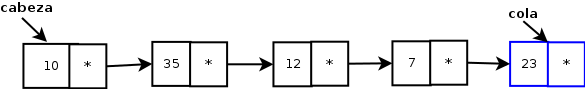
\includegraphics[scale=0.7]{Diagramas/RepresentacionColaNodosEnlazadosEncolar}
	\caption{Representación de la cola después de encolar el elemento 23}	
	\label{fig:cola-nodos-enlazados-encolar}
\end{figure}

En la linea 43 se aprecia el método \textbf{desencolar}. Lo primero que hace es preguntar si la cola no esta vacía (linea 45), en caso afirmativo, si cabeza es igual a cola significa que hay un sólo elemento, por lo tanto,  la \textit{cabeza} y \textit{cola} se les asigna null y de esta forma la cola quedaría vacía. Si \textit{cabeza} no es igual a \textit{cola}, significa que hay más de un elemento en la cola, por lo tanto, simplemente de desplaza la \textit{cabeza} al siguiente nodo (line 52). Finalmente se decrementa la variable \textit{tamanio} (indicando que hay un elemento menos en la cola).

A continuación el código de un Cliente que instancia la cola que hemos creado. En este caso se almacenan objetos de tipo entero, se encolan algunos números, se imprimen los valores del frente de la cola y se desencolan sus elementos.

\begin{lstlisting}[language=Java]
package co.unicauca.colas;
public class ClienteMain {
	public static void main(String[] args) {
		//Crear una nueva cola de enteros
		Cola<Integer> cola = new Cola<Integer>();
		//Se encolan algunos elementos
		cola.encolar(12);
		cola.encolar(13);
		cola.encolar(14);
		cola.encolar(15);
		//Se imprime el primer elemento de la cola
		System.out.println("El primer elemento de la cola es:" + cola.frente());
		
		cola.desencolar();
		System.out.println("El primer elemento de la cola es:" + cola.frente().toString());
		
		cola.desencolar();
		System.out.println("El primer elemento de la cola es:" + cola.frente());

		cola.desencolar();
		System.out.println("El primer elemento de la cola es:" + cola.frente());

		cola.desencolar();
		System.out.println("El primer elemento de la cola es:" + cola.frente());
 	}
}
\end{lstlisting}

La salida por consola de este programa sería la siguiente.

\begin{lstlisting}[numbers=none]
El primer elemento de la cola es: 12
El primer elemento de la cola es: 13
El primer elemento de la cola es: 14
El primer elemento de la cola es: 15
El primer elemento de la cola es: null
\end{lstlisting}

\section{La clase Queue de java}
La API de java ya trae implementada la cola mediante la interface \textit{java.util.Queu}. 

Las operaciones básicas son...

Entonces la pregunta que nos podemos hacer es, ¿si java ya trae una cola por qué implementar una propia mediante nodos enlazados? La respuesta es simple, porque implementando nuestra propia cola sabremos cómo funciona internamente una cola y habrá más aprendizaje. A continuación se muestra el mismo ejemplo de la sección Implementación del TAD en Java pero utilizando la interface Queue de java.

\begin{lstlisting}[language=Java]
/* Ejemplo del uso de la interface Queue*/
import java.util.Queue;
public class EjemploQueue{
    public static void main(String arg[]) {
        //Crea una nueva cola de enteros
        //FALTA CODIGO
    }
}
\end{lstlisting}


\section{Problemas que se resuelven con colas}
Las colas se utilizan en sistemas informáticos, transportes y operaciones de investigación (entre otros), donde los objetos, personas o eventos son tomados como datos que se almacenan y se guardan mediante colas para su posterior procesamiento. A continuación se describen problemas del mundo real donde la estructura fundamental se resuelve gracias a una cola.


\subsection{Simulador del despegue de aviones}
Se debe utilizar una cola para simular el despegue de aviones del aeropuerto el Dorado de Bogotá, las políticas que rigen las operaciones aéreas son las siguientes:
\begin{itemize}
\item Se tiene estimado que del aeropuerto pueden salir vuelos cada cinco minutos, siempre y cuando no hayan solicitudes de aterrizaje.
\item Un vuelo no puede salir del aeropuerto, antes de la hora programada.
\item Un vuelo no puede despegar del aeropuerto si se encuentran vuelos pendientes por despegar (se debe respetar la cola de vuelos).
\item El aeropuerto conoce con anterioridad la hora de salida de todos los vuelos programados para ese día. Las aerolíneas tienen programados vuelos con 10 minutos de diferencia.
\item Los aterrizajes ocurren de manera aleatoria. El aterrizaje tarda diez minutos (es prioritario el aterrizaje de un avión).
\item Se asume que la simulación inicia con mínimo 10 solicitudes de despegue.
\end{itemize}

A continuación un bosquejo de cómo podría ser la simulación.

\begin{lstlisting}[language=Java]
	public void simular(){
		//Crea la cola de vuelos
		Cola<Vuelo> cola = new Cola<Vuelo>();
		//Lee los vuelos desde el archivo y los carga en cola
		cola = leerVuelosDesdeArchivo();
		//Crea una instancia de tipo Proceso
		Proceso instancia = null;
		//Mientras haya procesos en la cola
	    while (!cola.esVacia()){
			instancia=cola.desencolar();
			if(hayAterrizaje()){
				//Simula el aterrizaje
			}else{
				//Simula el despeje
			}
		}
	}

\end{lstlisting}

\subsection{Simulador de la planificación de procesos round-robin}
Utilizando una cola de procesos, simular la planificación de procesos round-robin (turno circular) de un sistema operativo. A continuación se describe su funcionamiento.

Los sistemas operativos modernos permiten ejecutar simultáneamente dos o más procesos.  Cuando hay más de un proceso ejecutable, el sistema operativo debe decidir cuál proceso se ejecuta primero. La parte del sistema operativo que toma esta decisión se llama planificador; el algoritmo que usa se denomina algoritmo de planificación.  

El algoritmo de planificación de procesos Round Robin es uno de los más sencillos y antiguos REFERENCIA LIBRO SISTEMAS OPERATIVOS. A cada proceso se le asigna un intervalo de tiempo en la CPU, llamado cuanto, durante el cual se le permite ejecutarse. Si el proceso todavía se está ejecutando al expirar su cuanto, el sistema operativo se apropia de la CPU y se la da a otro proceso. Si el proceso se bloquea o termina antes de expirar el cuanto , se hace la conmutación de proceso. Para ello, el planificador mantiene una lista de procesos ejecutables. Cuando un proceso gasta su cuanto, se le coloca al final de la lista. A continuación un bosquejo de cómo podría ser la simulación.

\begin{lstlisting}[language=Java]
	public void simular(int cuanto){
		//Crea la cola de procesos
		Cola<Proceso> cola = new Cola<Proceso>();
		//Lee los procesos desde el archivo y los carga en cola
		cola = leerProcesosDesdeArchivo();
		//Crea una instancia de tipo Proceso
		Proceso instancia = null;
		//Simula el tiempo
		int tiempo=0;
		//Mientras haya procesos en la cola
	    while (!cola.esVacia()){
			instancia=cola.desencolar();
			System.out.println("Tiempo " + tiempo + ": " +  instancia.getId() + " entra a ejecucion);
			//Completar el codigo faltante
		}
	}
\end{lstlisting}

\section{Ejercicios Propuestos}
A continuación se plantean los siguientes ejercicios los cuales utilizan la estructura de datos Cola.

\begin{enumerate}
	\item Elabore una implementación en java del simulador del despegue y aterrizaje de aviones. Un archivo \textit{vuelos.txt} debe contener la programación ordenada por hora de salida de los vuelos de un día cualquiera. El formato debe ser así (numero de vuelo, aerolinea, horas, minutos), por ejemplo:\\
	10071,AVIANCA,7,0\\
	10072,AVIANCA,7,10\\
	10073,AVIANCA,7,20\\
	10073,SATENA,7,30\\
	10074,SATENA,7,40\\
	10075,AVIANCA,7,50\\
	10076,LAN,8,0\\
	10077,TAME,8,10\\
	10078,TAME,8,20\\
	
	Un ejemplo de la salida de la simulación podría ser:\\
	Despegue, vuelo:10071 Hora programada:7:00 Hora real:7:00\\
	Despegue, vuelo:10072 Hora programada:7:10 Hora real:7:10\\
	Aterrizaje a las 7:15\\
	Despegue, vuelo:10073 Hora programada:7:20 Hora real:7:25\\
	Despegue, vuelo:10073 Hora programada:7:30 Hora real:7:30\\
	Aterrizaje a las 7:35\\
	Aterrizaje a las 7:45\\
	Despegue, vuelo:10074 Hora programada:7:40 Hora real:7:55\\
	Aterrizaje a las 8:0\\
	Despegue, vuelo:10075 Hora programada:7:50 Hora real:8:10\\
	Despegue, vuelo:10076 Hora programada:8:00 Hora real:8:15\\
	Despegue, vuelo:10077 Hora programada:8:10 Hora real:8:20\\
	Despegue, vuelo:10078 Hora programada:8:20 Hora real:8:25\\
	Despegue, vuelo:10079 Hora programada:9:30 Hora real:8:30\\
	
	\item Elabore una implementación en java del simulador de la planificación de procesos round-robin. El programa debe simular la operación de la ejecución de procesos a partir de la información de un archivo de texto \textit{procesos.txt} que contiene la información básica de cada proceso (El nombre del proceso, el tiempo de ejecución).Un posible contenido de este archivo puede ser:\\
	P1, 100\\
	P2,15\\
	P3,40\\
	
	Una posible salida resultado de la ejecución de la simulación para un cuanto de 20 ms, con los tres procesos descritos anteriormente podría sería:\\
	Tiempo 0: P1 entra a ejecución. \\
	Tiempo 20: P1 se conmuta.  Pendiente por ejecutar 80 ms\\
	Tiempo 20: P2 entra a ejecución\\
	Tiempo 35: P2 se conmuta. Pendiente por ejecutar 0 ms\\
	Tiempo 35: P3 entra a ejecución\\
	Tiempo 55: P3 se conmuta. Pendiente por ejecutar 20 ms\\
	Tiempo 55: P1 entra a ejecución\\
	Tiempo 75: P1 se conmuta. Pendiente por ejecutar 60 ms\\
	Tiempo 75: P3 entra a ejecución\\
	Tiempo 95: P3 se conmuta. Pendiente por ejecutar 0 ms.\\
	Tiempo 95: P1 entre en ejecución\\
	Tiempo 155: P1 termina su ejecución\\
	Total tiempo de ejecución de todos los procesos:155 ms\\
	Total de conmutaciones: 4\\
\end{enumerate}

